\documentclass[11pt,a4paper]{article}
\usepackage{tikz}
\usetikzlibrary{arrows.meta,positioning}
\usepackage{tabularx}
\usepackage{amsmath,amssymb,amsthm}
\usepackage{geometry}
\geometry{margin=1in}
\usepackage{hyperref}
\usepackage{graphicx}
\usepackage{setspace}
\onehalfspacing

\title{\textbf{Paper B-04: Distributed and Cloud Computing:\\ A Constraint-Driven Flux Dynamics (CDFD) Perspective}}
\author{Steve Bico Mujjabi, MD\\
\small Independent Researcher\\
\small Founder, Vura Labs\\
\small Kampala, Uganda\\
\small ORCID: 0009-0001-0556-5516}
\date{August 2026}

\begin{document}
\maketitle

% BEGIN SHARED-METHODS POINTER
\noindent\textit{Shared Part IV notation and evidence boundaries are defined in \path{PART_IV_METHODS_AND_CLAIM_BOUNDARY.md}. This paper states only its local observables, comparison, and failure conditions.}
% END SHARED-METHODS POINTER


\begin{abstract}
This paper develops a falsifiable CDFD/AFL model of Distributed Compute. It maps tasks, data, synchronization, and user demand to driving flux $\Phi$, compute, memory, network, storage, and consistency limits to active constraint $C$, scheduling, replication, autoscaling, partitioning, and failover to responsiveness $S$, and queues, caches, checkpoints, state, and technical debt to structural memory $M_s$. The target outcome is latency, throughput, correctness, cost, and recovery, tested against traces, scheduler logs, dependency graphs, resource metrics, and failure injections. The paper treats universality as a shared model architecture rather than an assertion that unlike systems have the same material mechanism. It states the negative result that would make the mapping unnecessary and places the domain claim inside the cumulative CDFD programme and its reproducible runtime boundary.
\end{abstract}
% BEGIN CONSOLIDATION SCOPE
\section*{Consolidation Scope and Provenance}
This consolidated paper incorporates the distributed-computing and cloud-system scopes formerly carried by Papers B-04 and B-08. Queueing, utilization, latency, and failure recovery are compared against native systems-performance baselines.
% END CONSOLIDATION SCOPE


\section{Introduction}

A supercomputer or a cloud cluster is an engineered metabolic engine. It consumes electrical power and raw data, processes it through structured logic gates, and outputs highly ordered informational states. The fundamental challenge in distributed systems is load balancing: ensuring that no single node is overwhelmed while others sit idle.

In CDFD, this is a classic problem of managing a multi-node transport network. A distributed cluster is an active topological surface attempting to maintain a universal adaptive equilibrium across all its constituent parts.

\section{The Computational Adaptive Surface}
We govern the computational cluster using the Adaptive Operating Ratio:
\begin{equation}
    \Psi_s = \left( \frac{\Phi}{C} \right) \cdot S \cdot M_s
\end{equation}

For a specific server node within a cluster:
\begin{itemize}
    \item \textbf{Flux ($\Phi$)}: The incoming queue of computational tasks, data payloads, and requisite parallel synchronization signals.
    \item \textbf{Constraint ($C$)}: The physical limitations of the node, including CPU clock speed, RAM capacity, network bandwidth, and thermal throttling limits.
    \item \textbf{Responsiveness ($S$)}: The elasticity of the orchestration layer (e.g., Kubernetes) to dynamically spool up new containers, migrate processes, or adjust thread priority.
    \item \textbf{Memory ($M_s$)}: The rigidity of the software architecture. Legacy monolithic applications or rigid task schedulers represent high systemic memory. The cluster "remembers" its hardcoded instructions, resisting dynamic reallocation.
\end{itemize}

\subsection{Node Exhaustion and Cascading Latency}
In an optimal state, the orchestration layer perfectly matches incoming tasks to available nodes. The system operates efficiently at $\Psi_s \approx 1$.

Consider a sudden spike in highly complex, unoptimized queries ($\Phi$ surges). If the software architecture is rigidly monolithic (high $M_s$), the orchestrator cannot dynamically split the tasks across the cluster. The flux piles up on a few specific nodes. The constraints $C$ (RAM limits) are rapidly hit.

The adaptive ratio drops to $\Psi_s \ll 1$. The node begins "thrashing" (constantly swapping memory to disk), which reduces effective throughput. Because distributed tasks often require synchronous completion, the cluster can stall while waiting for the constrained node. The medical analogy is only structural: the engineering claim must be tested with queue, memory, and dependency telemetry.



\section{Measurement Layer}

% BEGIN PART IV MAJOR CROSS-DOMAIN UPGRADE
\section{Cross-Domain Model Upgrade: Mechanism, Scale, and Tests}

\subsection{Observable Translation}

The paper-specific translation begins with an observable chain rather than a
verbal analogy. For Distributed Compute, the proposed drive is tasks, data, synchronization, and user demand.
The active limitation is compute, memory, network, storage, and consistency limits. Responsiveness is carried by
scheduling, replication, autoscaling, partitioning, and failover, while retained state is represented by
queues, caches, checkpoints, state, and technical debt. The outcome to explain is latency, throughput, correctness, cost, and recovery.

\begin{table}[htbp]
\centering
\small
\caption{Operational CDFD/AFL map for Paper B-04.}
\begin{tabularx}{\textwidth}{|l|X|X|}
\hline
\textbf{Term} & \textbf{Paper-specific observable meaning} & \textbf{Measurement question} \\
\hline
$\Phi$ & tasks, data, synchronization, and user demand & What rate, load, gradient, or demand enters the focal system? \\
\hline
$C$ & compute, memory, network, storage, and consistency limits & Which measured bottleneck limits transfer, function, or recovery? \\
\hline
$S$ & scheduling, replication, autoscaling, partitioning, and failover & Which process changes effective capacity or reroutes the load? \\
\hline
$M_s$ & queues, caches, checkpoints, state, and technical debt & Which retained state makes equal present loads produce different futures? \\
\hline
$Y$ & latency, throughput, correctness, cost, and recovery & Which outcome is predicted out of sample, with uncertainty? \\
\hline
\end{tabularx}
\end{table}

\begin{figure}[htbp]
\centering
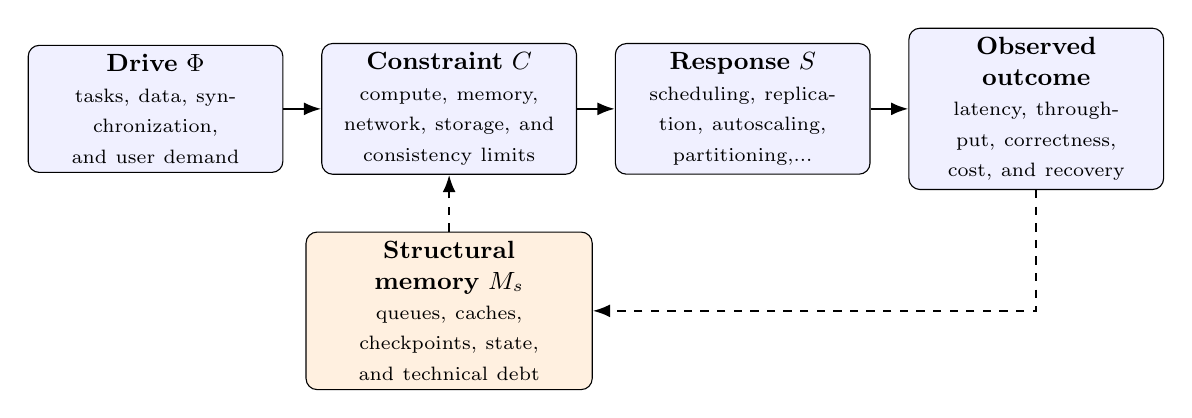
\begin{tikzpicture}[
    node distance=0.48cm,
    every node/.style={font=\small},
    box/.style={draw, rounded corners, align=center, minimum height=1.45cm, text width=3.0cm, fill=blue!6},
    memory/.style={draw, rounded corners, align=center, minimum height=1.25cm, text width=3.4cm, fill=orange!12},
    flow/.style={-{Latex[length=2.2mm]}, thick},
    feedback/.style={-{Latex[length=2.2mm]}, thick, dashed}
]
\node[box] (drive) {\textbf{Drive $\Phi$}\\\scriptsize tasks, data, synchronization, and user demand};
\node[box, right=of drive] (constraint) {\textbf{Constraint $C$}\\\scriptsize compute, memory, network, storage, and consistency limits};
\node[box, right=of constraint] (response) {\textbf{Response $S$}\\\scriptsize scheduling, replication, autoscaling, partitioning,...};
\node[box, right=of response] (outcome) {\textbf{Observed outcome}\\\scriptsize latency, throughput, correctness, cost, and recovery};
\node[memory, below=0.72cm of constraint] (memory) {\textbf{Structural memory $M_s$}\\\scriptsize queues, caches, checkpoints, state, and technical debt};
\draw[flow] (drive) -- (constraint);
\draw[flow] (constraint) -- (response);
\draw[flow] (response) -- (outcome);
\draw[feedback] (outcome.south) |- (memory.east);
\draw[feedback] (memory.north) -- (constraint.south);
\end{tikzpicture}
\caption{Paper B-04 observable CDFD/AFL architecture for Distributed Compute. Solid arrows give the proposed forward chain; dashed arrows make history-dependent feedback explicit.}
\label{fig:b04-architecture}
\end{figure}

\subsection{Paper-Specific Causal Hypothesis}

For this paper, the hypothesized causal sequence is specific. A change in
tasks, data, synchronization, and user demand arrives faster than scheduling, replication, autoscaling, partitioning, and failover can compensate.
This raises or redistributes compute, memory, network, storage, and consistency limits. If the load persists,
the retained state encoded by queues, caches, checkpoints, state, and technical debt changes the next response, so a later event of equal
magnitude can produce a different trajectory in latency, throughput, correctness, cost, and recovery. The
scientific task is to estimate that sequence against the best ordinary model of
the domain, not merely to redescribe the outcome after it occurs.

\subsection{Cross-Scale Translation Without Mechanistic Erasure}

For the engineered systems family, the cross-domain translation compares demand, designed capacity, feedback control, dependency topology, and accumulated technical state. The strongest engineering use is prospective: the mapping must identify a bottleneck, a control action, or a recovery signature before the failure occurs. \cite{BarabasiAlbert1999,WattsStrogatz1998,Shannon1948,BakTangWiesenfeld1987}
The required scale declaration for this paper is nanoseconds to years; processes to global services. At short
scales, the key question is whether the incoming drive is transmitted,
buffered, or diverted. At intermediate scales, response changes effective
capacity and network exposure. At long scales, retained structure can alter the
state space itself. A result is genuinely cross-scale only when the aggregation
rule is stated and the same conclusion is not an artifact of averaging.

\subsection{Evidence Ladder and Discriminating Tests}

\begin{table}[htbp]
\centering
\small
\caption{Evidence ladder for Paper B-04. Each rung can fail independently.}
\begin{tabularx}{\textwidth}{|p{0.17\textwidth}|X|X|}
\hline
\textbf{Test} & \textbf{Design} & \textbf{Discriminating result} \\
\hline
Proxy audit & Measure traces, scheduler logs, dependency graphs, resource metrics, and failure injections and preregister how each record maps to $\Phi$, $C$, $S$, $M_s$, and $Y$. & The mapping fails if proxies are non-identifiable, circular, or change meaning across cases. \\
\hline
Load ramp & Apply or observe a burst load combined with a node or network partition while estimating the dominant constraint and response time. & A threshold claim requires a reproducible nonlinear change and uncertainty bounds, not a visually chosen breakpoint. \\
\hline
Recovery and memory & Match present load across units with different histories, then compare recovery paths. & The memory claim requires history-dependent divergence after current conditions are controlled. \\
\hline
Model comparison & Compare the baseline domain model with and without the CDFD/AFL state variables using held-out data. & The paper's stated falsifier is: the added state variables do not improve performance or failure prediction. \\
\hline
\end{tabularx}
\end{table}

\subsection{Research Programme and Boundary Conditions}

The immediate research programme has four steps. First, construct a documented
dataset from traces, scheduler logs, dependency graphs, resource metrics, and failure injections and retain raw units before normalization.
Second, fit a baseline domain model and report its calibration and out-of-sample
error. Third, add the smallest identifiable CDFD/AFL state extension and test
whether it improves prediction of latency, throughput, correctness, cost, and recovery. Fourth, repeat the
analysis across the declared scale range and publish negative cases as part of
the cross-domain translation audit.

% END PART IV MAJOR CROSS-DOMAIN UPGRADE

\section{Conclusion}
Distributed computing is an exercise in applied thermodynamics. By viewing server clusters through the CDFD lens, engineers can move beyond static load balancing and design "liquid" architectures where the software constraints ($C$) and memory ($M_s$) actively mutate in real-time to absorb turbulent informational flux, mirroring the plasticity of a biological neural network.
\section*{Conflict of Interest} The author declares no conflict of interest.
\section*{Data Availability}
Part-specific runtime diagnostics are under each Part's \path{outputs/} directory.

Release-wide code: \path{Part_E_Synthesis/supplementary/}.

Generated summaries: \path{Part_E_Synthesis/outputs/}.

Figures: \path{Part_E_Synthesis/figures/}.


\section{Reference Layer}
\bibliographystyle{plain}
\bibliography{universal_afl_references}
\end{document}
